% template.tex, dated April 5 2013
% This is a template file for Annual Reviews 1 column Journals
%
% Compilation using ar-1col.cls' - version 1.0, Aptara Inc.
% (c) 2013 AR
%
% Steps to compile: latex latex latex
%
% For tracking purposes => this is v1.0 - Apr. 2013

\documentclass[a4paper]{ar-1col}


\usepackage[comma]{natbib,amssymb}

\setcounter{secnumdepth}{4}

% Metadata Information
\jname{Annu. Rev. Astron. Astrophys.}
\jvol{58}
\jyear{2020}
\doi{10.1146/((please add article doi))}

%\bibliographystyle{ar-style2.bst}
\bibliographystyle{aasjournal.bst}

% Document starts
\begin{document}

% Page header
\markboth{Andrews}{Disk Structures}

% Title
\title{Observing the Structures of Protoplanetary Disks}


%Authors, affiliations address.
\author{Sean M. Andrews
\affil{Center for Astrophysics \textbar\ Harvard \& Smithsonian \\ Cambridge, Massachusetts, USA 02138; email: sandrews@cfa.harvard.edu}}

%Abstract
\begin{abstract}
Debris disks are tenuous, dust-dominated disks commonly observed around
stars over a wide range of ages. Those around main sequence stars are analogous
to the Solar System’s Kuiper Belt and zodiacal light. The dust in debris
disks is believed to be continuously regenerated, originating primarily with
collisions of planetesimals. Observations of debris disks provide insight into
the evolution of planetary systems; and the composition of dust, comets,
and planetesimals outside the Solar System; as well as placing constraints
on the orbital architecture and potentially the masses of exoplanets that are
not otherwise detectable. This review highlights recent advances in multiwavelength,
high-resolution scattered light and thermal imaging that have
revealed a complex and intricate diversity of structures in debris disks and
discusses how modeling methods are evolving with the breadth and depth of
the available observations. Two rapidly advancing subfields highlighted in
this review include observations of atomic and molecular gas around main
sequence stars and variations in emission from debris disks on very short
(days to years) timescales, providing evidence of non-steady-state collisional
evolution particularly in young debris disks.
\begin{itemize}
\item First finding.
\item Second finding.
\item Third finding.
\end{itemize}
\end{abstract}

%Keywords, etc.
\begin{keywords}
keywords, separated by comma, no full stop, lowercase
\end{keywords}
\maketitle

%Table of Contents
\tableofcontents


\section{INTRODUCTION} \label{sec:intro}

\subsection{Motivation} \label{sec:motivation}

The formation and early evolution of a star and its planets are fundamentally governed by their relationships with a circumstellar disk.  The telltale signatures of the foundational interactions between disk, star, and planets are imprinted on the disk structure -- the detailed spatial distribution and physical conditions of the disk material.  Measurements of disk structures, complemented with theoretical simulations, can be used to figure out how the key physical mechanisms associated with star and planet formation operate. 

Star formation begins with the gravitational collapse of an over-density (core) in a molecular cloud.  Rotation of that core implies that material from its outer regions, with higher angular momentum, is channeled onto a flattened disk that orbits a central protostar, rather than directly onto the star itself \citep{cassen81,terebey84}.  In that sense, disks are a simple consequence of angular momentum conservation.  Measurements of young disk structures, still embedded in their natal core material (envelope), reveal much about the star formation process: their sizes help distinguish the roles that magnetic fields have in regulating core collapse; their masses constrain the typical protostellar accretion rates; and their density distributions encode the mechanics of angular momentum transfer and accretion that ultimately determine the stellar mass.  

Disks are also the birthplaces of planetary systems.  The prevalence, formation modes, masses, orbital architectures, and compositions of planets depend intimately on the physical conditions in the disk at their formation sites, the evolution of that disk structure (locally and globally), and the planetary migration driven by dynamical interactions with the disk material.  Measurements of the disk mass and its spatial distribution offer crucial boundary conditions for models of planet formation.  Combined with the demographic properties observed in the mature exoplanet population, that information can help develop and refine a predictive formation theory, despite the considerable complexity of the associated physical processes \citep[e.g.,][]{ida04,alibert05}.



\subsection{Observational Primer} \label{sec:primer}

In many ways, disk structures offer profound insights on how the properties of stars and planetary systems are shaped by their origins.  This review is focused on the recent landscape of observational constraints on disk structures: how relevant measurements are made, what they suggest about disk properties, and how those properties are connected to star and planet formation.  The key measurements of disk structures require high angular resolution data, as the typical disk in a nearby star-forming region subtends only $\sim$1$^{\prime\prime}$ on the sky.  Most of any given disk is relatively cool enough (temperatures $<$100 K) that it emits most efficiently in the millimeter-wave part of the spectrum (hereafter mm, meaning $\lambda \approx 0.5$--5 mm).  Coupling these small angular sizes and cool temperatures, considerable emphasis in this review will be placed on radio interferometry as an essential tool.  Indeed, dramatic progress over the past decade has largely been driven by the commissioning of the transformational Atacama Large Millimeter/submillimeter Array (ALMA) facility.
\begin{marginnote}[]
\entry{sub-mm}{$\lambda \approx 0.1$--0.5 mm, $\nu \approx 0.6$--3 THz.}
\entry{mm}{$\lambda \approx 0.5$--5 mm, $\nu \approx 60$--600 GHz.}
\entry{cm}{$\lambda \approx 5$--50 mm, $\nu \approx 6$--60 GHz.}
\end{marginnote}

Three categories of observational tracer are useful for studying disk structures: scattered light, thermal continuum emission, and (primarily molecular) spectral line emission.  The first two are sensitive to the physical conditions and distribution of solids, and the third is used to measure the properties of the gas.  Each observational probe is sensitive to different materials and physical conditions, ensuring considerable diversity in the disk appearance when viewed in different tracers.  An illustrative example is shown in {\bf Figure \ref{fig:ims}}. 


\subsubsection{Scattered Light} \label{sec:primer_scat}
Small ($\mu$m-sized) dust grains suspended in the disk atmosphere can reflect the optical and infrared radiation emitted by the the central host star.  This scattered light is especially sensitive to the vertical distribution of the dust, and how it changes with radius \citep[e.g.,][]{debes13,stolker16,garufi17}.  Spectral and polarization variations in the scattered light morphology can constrain the albedo and phase function of the scatterers, which are set by the size, shape, and composition of the grains \citep{debes08,min12,min16}.  Aside from uniquely probing the dust disk surface geometry, the key advantage of this tracer is resolution: adaptive optics systems operating at the diffraction limit on 8--10 m telescopes measure features at 30--50 mas scales ($\sim$5 au).  The important challenges are contrast with the host stars, which prevent measurements in the innermost disk ($\lesssim 10$ au), and sensitivity at large radii, due to the dilution of the stellar radiation field.  The latter issue has limited the sample of resolved scattered light measurements, and biased it toward disks with brighter (earlier type) hosts.    

%The continuum and line emission are thermal radiative processes, so the kind of information about the disk structure available from a given tracer depends on its optical depth, $\tau_\nu$.  If the tracer emission is optically thin ($\tau_\nu \ll 1$), the intensity scales roughly with the product $I_\nu \propto X B_\nu(T) N$, where $B_\nu(T)$ is the Planck function at the local temperature, $N$ is column density, and $X$ is a (potentially complicated) conversion factor that quantifies how much emission is produced per unit mass for that tracer species.  With some information on $X$, $T$, and the disk geometry, a measurement of $I_\nu$ offers a density constraint.  If the emission is optically thick ($\tau_\nu \gtrsim 1$), the intensity scales with the temperature at the effective photosphere of the tracer, $I_\nu \propto B_\nu(T)$.  In this case, only lower bounds on the densities of the tracer species are available, and the emission can be affected by scattering.          

\begin{figure}[t]
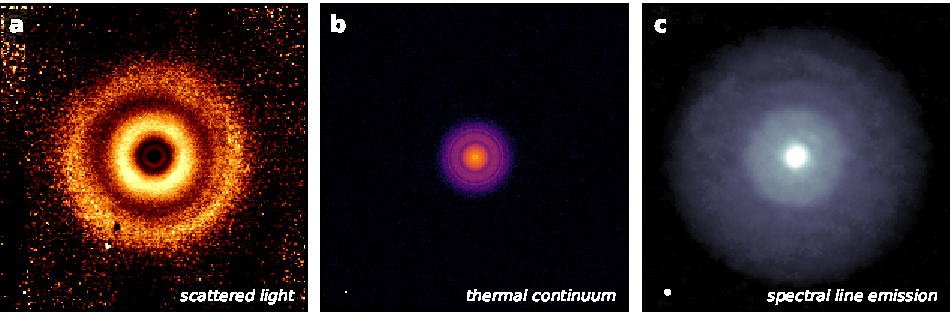
\includegraphics[width=\textwidth]{twhya_gallery.pdf}
\caption{Images of the disk around TW Hya in (a) 1.6 $\mu$m scattered light \citep{vanboekel17}, (b) 0.9 mm thermal continuum \citep{andrews16}, and (c) the $^{12}$CO $J$=3$-$2 emission line \citep{huang18}.  The spatial scales are the same in each panel (300 au on a side); the FWHM resolution for each image is shown as an ellipse in the lower left corner of each, but is generally too small to be easily visible.  This gallery illustrates how the appearance of the disk structure varies considerably with the observational tracer.}
\label{fig:ims}
\end{figure}


\subsubsection{Continuum Emission} \label{sec:primer_cont}
Disk solids also emit their own thermal continuum radiation that spans at least four decades in wavelength (from 1 $\mu$m to 1 cm).  Most of that emission is optically thick, and therefore a diagnostic of the temperature structure in the disk \citep[e.g., see][]{andrews15}.  Lower optical depths ($\tau_\nu$) are available at longer wavelengths, with the transition to optically thin traditionally expected in the sub-mm.  In the optically thin limit ($\tau_\nu \ll 1$), the continuum intensities scale with the product $I_\nu \propto \kappa_\nu B_\nu(T) \Sigma_s$, where $\kappa_\nu$ is the opacity (absorption cross section per unit mass), $B_\nu(T)$ the Planck function at the local temperature $T$, and $\Sigma_s$ the surface density of solids.  The mm continuum spectrum has a roughly power-law shape, $I_\nu \propto \nu^{\alpha_{\rm mm}}$, with the spectral index set by the sum of contributions from the Planck function ($B_\nu \propto \nu^{\alpha_{\rm Pl}}$, where $\alpha_{\rm Pl} \approx 1.7$--2.0 for $T > 15$ K) and the opacity spectrum ($\kappa_\nu \propto \nu^\beta$), so $\alpha_{\rm mm} \approx \alpha_{\rm Pl} + \beta$ \citep{beckwith91,ricci10a,ricci10b}.  The opacity index, $\beta$, depends on the sizes, shapes, and compositions of the solids \citep{miyake93,dalessio01,draine06}.  

In principle, resolved measurements of the mm continuum provide an ideal opportunity to constrain the mass distribution (and particle properties) of the disk solids.  This broadband tracer is also relatively easy to observe at high resolution, down to 10--20 mas scales ($\sim$2 au; and no contrast issues with the host), thanks to the sensitivity and resolution of ALMA.  This means measurements are plentiful: much of the collective knowledge of resolved disk structures is based on mm continuum data.  There are two key ambiguities in interpreting these data.  First, some of the emission is likely optically thick, perhaps preferentially in the inner disk \citep[see][]{beckwith90,aw05}.  In that case, the intensities saturate to $B_\nu(T)$ and the spectral index reverts to $\alpha_{\rm Pl}$.  Self-scattering could diminish the intensities below $B_\nu(T)$ and permit $\alpha_{\rm mm}$ to vary in the range 1.5--2.5, depending on the frequency dependence of the albedo \citep{zhu19,liu19}.  And second, our relative ignorance of the microphysical particle properties that set $\kappa_\nu$ -- their mineralogical (and ice) compositions \citep{pollack94}, sizes \citep{miyake93}, and structures \citep{henning96} -- means that links between the emission and physical conditions are intrinsically uncertain, even when optical depths are low.


\subsubsection{Spectral Line Emission} \label{sec:primer_lines}
The dominant constituent by mass in a disk is cold H$_2$ gas.  But, H$_2$ lacks a permanent dipole moment and is therefore essentially `dark': there is no direct probe of the gas mass reservoir.  Instead, constraints on the structure of the gas disk rely on spatially and spectrally resolved measurements of trace molecular rotational transitions throughout the (sub-)mm bands.  Such emission lines can be optically thick or thin.  Like the continuum, optically thick line emission has $I_\nu \propto B_\nu(T)$ (where $T$ is formally the excitation temperature, equivalent to the gas temperature in local thermodynamic equilibrium, LTE): the key difference is that the line photosphere (where $\tau_\nu \sim 1$) can be located at a higher altitude above the midplane than the continuum \citep{beckwith93}.  For low optical depths, the line intensity scales with the product of the abundance of molecules of that species, the surface density of the gas, and the temperature, $I_\nu \propto [{\rm X}/{\rm H}_2] \Sigma_g B_\nu(T)$.  In either case, the spatio-kinematic morphology of the line emission is set by the gas dynamics, dominated by Keplerian rotation around the host star \citep{marsh92,koerner93}.  The line width is determined by thermal and non-thermal broadening contributions; the latter is typically associated with turbulence \citep{hughes11}.         

Resolved measurements of multiple optically thick lines with a range of critical densities can be used to trace the temperature structure of the disk atmosphere \citep[e.g.,][]{dartois03}, and optically thin lines can theoretically be used to constrain gas densities.  With sufficient spectral resolution, such emission line datasets can be used to tomographically reconstruct the disk velocity field \citep{simon00,rosenfeld13a} and assess the level of turbulence \citep{guilloteau12,flaherty15}.  ALMA is in principle capable of resolving such line emission at tens of milliarcsecond scales ($\sim$2--5 au) in few m s$^{-1}$-wide velocity channels, but the narrow bandwidths and relatively low abundances of trace molecular species mean that sensitivity is a perennial challenge (particularly when optical depths are low).  Accordingly, line measurements of disks with the requisite sensitivity and resolution are considerably less common than for the continuum.  The two most prominent challenges in interpreting spectral line data are confusion with the emitting layer location (in the typical case where resolution is limited) and the large (potentially orders of magnitude) uncertainties in the molecular abundances (relative to H$_2$).         
%In the literature, two tracer molecule options have been considered for $M_g$ constraints: HD (the primary isotopologue of H$_2$) and CO.  The advantage of HD is the simplicity of its associated chemical network, meaning the HD/H$_2$ abundance ratio is known well \citep{bergin13,mcclure16,trapman17}.  But with a ground state transition in the far-infrared (112 $\mu$m), HD measurements are scarce (and currently inaccessible).  CO is a popular alternative, but the rotational lines from the primary isotopologue are very optically thick \citep{beckwith93}.  Therefore, gas mass estimates rely on line luminosity measurements of rarer isotopologues, usually $^{13}$CO and C$^{18}$O together \citep{williamsbest14}.  The advantages of CO tracers are practical, since these lines are (relatively) bright and accessible (with a sequence of transitions throughout the microwave spectrum), but their abundances are more uncertain.  For reference, the utility of a suite of (less favorable) alternative tracers for $M_g$ measurements were explored by \citet{molyarova17}.




\subsection{Statement of Scope} \label{sec:scope}

Keeping in mind the foundational motivations for measuring disk structures, and the observational tools that are available, this review covers four broad (and inter-related) topics that currently occupy much of the effort in the disk community: (1) the inferred key properties of disk structures and their associated ambiguities (Section \ref{sec:structure}); (2) the constraints on evolutionary and environmental dependencies based on demographics studies (Section \ref{sec:demographics}); (3) the evidence for (and problems with) the growth and migration of disk solids (Section \ref{sec:solids}); and (4) the properties and roles of small-scale {\it substructures} in shaping observables and facilitating planet formation (Section \ref{sec:substructures}).  The review concludes with a summary that aims to distill the findings for these topics and reflect the current state of the field (Section \ref{sec:summary}), as well as a discussion of some potentially fruitful avenues for future work (Section \ref{sec:future}).  




\section{KEY\ STRUCTURE\ PROPERTIES} \label{sec:structure}

The spatial distribution of mass -- the density structure -- is without question the fundamental property of interest for disks.  The over-arching conceptual design of the field presumes that disk evolution is basically deterministic, such that a collection of ``snapshots" of disk density distributions that span an appropriate range of environmental and evolutionary states could be used to work out the mechanics of key physical processes and thereby refine a predictive model of how disks regulate star and planet formation.  This section of the review is focused on the underlying motivations, observational constraints, and lingering ambiguities associated with the mass distributions in disks (Sections \ref{sec:mass}--\ref{sec:sigma}).  Because most probes of disk structures to date rely on their solids, special attention is paid to the continuum opacities and their links to particle properties (Section \ref{sec:opacities}).  The intrinsic connections (physical and observational) between the density structure and the thermal and dynamical state of the disk material are summarized in Section \ref{sec:temp} and \ref{sec:turb}, respectively.        

\begin{textbox}[t]\section{Notation, Conventions, and Nomenclature}
To set the practical framework for interpreting the results in this field, some discussion of standards and terminology is helpful.  The common characterization of the density structure in disks essentially condenses to a one-dimensional description through the radial surface density profile, $\Sigma$, defined such that the mass $M = 2\pi \int \Sigma \, r \, dr$.  This is not intended to diminish the azimuthal or vertical dimensions (with coordinates $\varphi$ and $z$, respectively), but rather reflects both a convenient simplification and the fact that disks are by their nature geometrically thin.  Because of their different physical and observable behaviors, it is also useful to differentiate the disk contents into two broad categories, solids and gas; their density profiles are related by the (vertically averaged) solids-to-gas ratio, $\zeta = \Sigma_s / \Sigma_g$.  The goals of this section are to motivate the physical interest in $\Sigma_s$ and $\Sigma_g$, establish the related observable properties, summarize the state of measurements, review some important limitations, and outline the links to the thermal and dynamical structures of disks.  
\end{textbox}



\subsection{Masses} \label{sec:mass}

Much of the emphasis in the field is on the integrated quantity, the disk mass, rather than the density distribution.  That is mostly a practical limitation, but many of the key insights and issues can be illustrated well from this coarser perspective.  The primary interest is that measurements of disk masses offer elementary constraints on the contents of planetary systems.  Summing the terrestrial planet and giant planet core masses offers a conservative lower bound on the solid mass of the Solar Nebula disk ($M_s > 45 M_\oplus$; \citealt{weidenschilling77}) or its exoplanet counterparts \citep[e.g.,][]{chiang13}.  Extrapolations of the current planetary atmosphere contents to the primordial H,He-rich gas expected in disks \citep[e.g.,][]{kusaka70} enable an analogous limit for the gas masses ($M_g > 0.01 M_\odot$; e.g., \citealt{hayashi81}).  The current census of exoplanets finds an abundance of worlds orbiting other stars \citep{howard10,dressing13}, but the efficiency of the metamorphosis of disk material into planetary systems is unclear without a comparison of the mass reservoirs in the parent and descendent populations.          


\subsubsection{Overview of Measurements}
While disk solids are a minor contributor to the total mass budget (with a disk-averaged $\langle \zeta \rangle \approx 0.01$), the crucial roles they play in all aspects of disk evolution and planet formation justify special attention to their mass reservoir, $M_s$.  As discussed in Section \ref{sec:primer_cont}, the luminosity of the mm continuum emission should scale roughly with $M_s$.  The advent of bolometer detectors on single-dish telescopes motivated a series of photometry surveys designed to measure $M_s$ for hundreds of disks starting 30 years ago \citep{weintraub89,beckwith90,andre94,osterloh95,aw05,aw07b}, and continuing today with more sensitive interferometers \citep[e.g.,][]{andrews13,ansdell16,cieza19}.  The measured luminosity (hereafter $L_{\rm mm}$) distribution spans at least three decades and, though clearly influenced by observational and physical selection effects (Section \ref{sec:demographics}), it provides some rough guidance on $M_s$ values.  For standard assumptions about the disk-averaged temperature ($\langle T \rangle \approx 20$ K, based on crude models of infrared emission; \citealt{aw05}) and opacity ($\langle \kappa_\nu \rangle \approx 2.3$ cm$^2$ g $^{-1}$ at $\lambda = 1.3$ mm, as asserted by \citealt{beckwith90}), these luminosities imply a range $M_s \approx 1$--1000 $M_\oplus$.
% additional photometry surveys: 
% single-dish = reipurth93, henning93, jensen94, jensen96, nurnberger98, cieza15, ansdell15; 
% interferometry = williams05, mann09, mann10, mann14, mann15, harris12, akeson14, akeson19, carpenter14, pascucci16, vanderplas16, barenfeld17, ansdell17, law17, eisner06, eisner08, eisner16, cox17, eisner18, ward-duong18, ruiz-rodriguez18

There are many fewer estimates of gas masses, $M_g$, owing to the intrinsically more challenging observations of the emission line tracers (Section \ref{sec:primer_lines}).  In the literature, two tracer molecule options have been considered for $M_g$ constraints: HD (the primary isotopologue of H$_2$) and CO.  The advantage of HD is the simplicity of its associated chemical network, meaning the HD/H$_2$ abundance ratio is known well \citep{bergin13,mcclure16,trapman17}.  But with a ground state transition in the far-infrared (112 $\mu$m), HD measurements are scarce (and currently inaccessible).  CO is a popular alternative, but the rotational lines from the primary isotopologue are very optically thick \citep{beckwith93}.  Therefore, gas mass estimates rely on line luminosity measurements of rarer isotopologues, usually $^{13}$CO and C$^{18}$O together \citep{williamsbest14}.  The advantages of CO tracers are practical, since these lines are (relatively) bright and accessible (with a sequence of transitions throughout the microwave spectrum), but their abundances are more uncertain.  For reference, the utility of a suite of (less favorable) alternative tracers for $M_g$ measurements were explored by \citet{molyarova17}.  The ground state HD emission line has been detected from only three disks, suggesting $M_g \ge 0.01 M_\odot$ based on detailed models of their thermal structures \citep{bergin13,mcclure16}.  Larger samples of CO isotopologue emission line luminosities typically infer considerably lower values, $M_g < 0.001 M_\odot$ \citep[and detection rates are relatively low; e.g.,][]{ansdell16,long17}, when referenced to an extensive grid of model structures that assumes the CO/H$_2$ abundance in disks is comparable to the interstellar medium \citep{williamsbest14}.     


\subsubsection{Caveats and Ambiguities}
Section \ref{sec:primer} outlines the key sources of ambiguity in the (continuum or spectral line) tracers of mass: some of the emission may be optically thick (so the intensity saturates and mass is hidden), and the exchange rate between optically thin emission and mass can be considerably uncertain.  The first of these implies that masses could be underestimated.  Insight on the severity of this ambiguity is available with measurements of the surface area of the optically thick contamination, which will be revisited in various contexts below.  The second issue largely reflects our limited knowledge of the particle properties (manifested in $\kappa_\nu$) in the reservoir of solids or the chemical evolution (manifested in [${\rm X}/{\rm H}_2$]) in the gas phase, although uncertainties in the thermal structure also play a part (see Section \ref{sec:temp}).  Uncertainties in the opacities are significant enough in various aspects of the field that they merit their own discussion (Section \ref{sec:opacities}).           

%Shifting attention to the gas mass, there are direct analogues of these same ambiguities.  First, there is also the concern that the optically thin approximation is at least partially invalid, particularly for the HD and $^{13}$CO lines, implying again that mass may be hidden ($M_g$ is under-estimated).  As with the microwave continuum, the emission from an optically thin spectral line traces the produce of temperature and column density (i.e., mass).  The key difference is that the line emission originates from a more two-dimensional geometry (radial and vertical), which can potentially incorporate pronounced temperature gradients that are directly related to the distribution of the tracer abundances.  This is especially significant for $M_g$ estimates from the HD ground state line, which by a quirk of its excitation physics has an exponential $T$ dependence \citep{bergin13}.  In any case, a good model or measurement of $T(r, z)$ is required for a robust estimate of $M_g$ (see Section \ref{sec:temp}).    

The $M_g$ ambiguities associated with the abundances of tracer molecules can be significant.  For HD, the  chemical network is simple enough that the gas phase abundance should be fairly robust; the open questions are related to the unaccounted contribution of enhanced D fractionation in ices or hydrocarbons that could lead to an under-estimate of HD/H$_2$ (and therefore $M_g$).  The situation with CO is more complicated.  Presuming the interstellar CO/H$_2$ abundance ratio and isotopic fractionation \citep{frerking82}, the observed CO isotopologue luminosities from disks suggest surprisingly low $M_g$ values (by a factor of $\sim$5--10; \citealt{williamsbest14}) relative to other gas tracers in the same disks \citep{chapillon10,favre13,kama16a} or estimates of $M_s$ and presumed interstellar solids-to-gas ratios ($\zeta \approx 0.01$; \citealt{kastner97,dutrey03,ansdell16,long17}).  This apparent anomaly can be reconciled by invoking a higher solids-to-gas ratio ($\zeta \ge 0.1$) or modifying the assumed abundances.  The right direction and amplitude of abundance changes are expected from various chemical processes, including adsorption onto solids (freezeout; \citealt{aikawa97,aikawa02,dutrey97}), isotope-selective photodissociation \citep{visser09,miotello14,miotello16}, or C and O sequestration into other species (e.g., CO$_2$ ice, complex organics; \citealt{reboussin15,yu17a,miotello17,bosman18,dodson-robinson18}).

The salient point is that the adoption of standard abundance ratios is more or less designed to offer lower limits on $M_g$.  Depending on the tracer, those estimates could in principle be too low by a factor of a few (HD) to several orders of magnitude (CO isotopologues).  An analogous choice routinely made for the standard mm opacities (see Section \ref{sec:opacities}) means that the same is true for estimates of $M_s$.


%there is the subtle, added complication of the continuum too (optically thick line-blocking, and even subtraction issues a la weaver).  so, you also sort of want a good model of the continuum (ugh).



\subsection{Sizes} \label{sec:sizes}

The first step in progressing from total mass measurements to resolved density profiles is through estimates of disk sizes.  There is no obvious general definition for size from an observational perspective, since any metric depends on the prescription adopted for interpreting the radial variation of a given tracer.  There is an expectation that the mass distribution exhibits a break at some radius, beyond which it drops off more precipitously into the background.  That practical notion was originally motivated by the sharp cut-off of larger bodies in the Solar System around 40 au \citep[e.g.,][]{luu02}, but it is now supported by many disk observations \citep[e.g.,][]{andrews18}.  Nevertheless, there is no {\it a priori} knowledge of the detailed behavior of that transition, nor how it manifests in different tracers.  The ideal solution would be to employ a robust parametric model for the physical structure and use that to homogenize size measurements.  But it should be clear at this point that such an effort is littered with ambiguities.  Recognizing that ignorance for the time being, the more practical approach is to assign an empirical definition of size as the effective radius that encircles some fixed fraction of the tracer luminosity. 


\subsubsection{Overview of Measurements}
Resolved size measurements of the $\lambda \approx 1$ mm continuum emission from solids are available for more than 100 nearby disks, with radii in the range $\sim$5--200 au (\citealt{tripathi17,tazzari17,andrews18}, Hendler et al.~2019).  Coarser constraints find similar values for another $\sim$100 targets \citep[e.g.,][]{barenfeld17_sizes,eisner18,cieza19}.  The lower bound of this range is presumably limited by resolution.  In general, there is a tight correlation between the continuum sizes and luminosities \citep{andrews10,pietu14} with a scaling relation $L_{\rm mm} \propto R_{\rm mm}^{1/2}$ \citep{tripathi17,andrews18}, although this may flatten out at the low end or exhibit some other demographic dependence (Hendler et al.~2019; see Section \ref{sec:demographics}).  {\bf Figure \ref{fig:sizes}} shows the this size--luminosity scaling behavior.  This relationship is presumably produced by the evolution of disk solids \citep{tripathi17,rosotti19b}, although extracting more information in that context is potentially muddled by a degeneracy with high optical depths \citep{andrews18,zhu19}.  

The spatial variation of the mm spectrum shape suggests that the continuum size is correlated with the observing frequency (e.g., \citealt{perez12,lperez15,tazzari16}).  The context of such inferences will be revisited elsewhere (see Section \ref{sec:solids}), but explicit estimates of the shape of this correlation indicate a modest scaling, $R_{\rm mm} \propto \nu^{0.2-0.5}$ \citep[e.g.,][]{tripathi18}.  An alternative size metric for the solids is available from the extent of the optical/infrared starlight scattered off the disk surface.  Despite the difficulties of measuring that signal at large distances from the star, the current suite of scattered light images clearly indicate that the $\mu$m-sized dust grains that reflect starlight are distributed out to considerably large distances than the larger particles responsible for the mm continuum ({\bf Figure \ref{fig:ims}} illustrates this with a particularly clear example).  

Owing to limited sensitivity, there are many fewer size measurements in spectral line tracers of the gas.  The $^{12}$CO lines typically extend to radii of $\sim$100--500 au \citep{ansdell18}, although there are a few exceptional outliers on the high end \citep[e.g.,][]{guilloteau98,panic09}.  Smaller disks presumably exist, but are weak enough line emitters that they are missing in current samples \citep[e.g.,][]{barenfeld17_sizes}.  Nevertheless, tracer size comparisons for individual disks make it clear that the spectral line emission extends typically twice as far from the host star as the microwave continuum (\citealt{ansdell18}; see {\bf Figure \ref{fig:sizes}}).  Some of that size discrepancy is produced by the different optical depths of the tracers \citep{hughes08,trapman19}, but detailed modeling efforts have convincingly argued for a genuine variation between the tracer densities as well \citep[e.g.,][]{panic09,andrews12,degregorio-monsalvo13,rosenfeld13b,facchini17}.  The implication is a radial decrease in the solids-to-gas ratio ($\zeta$), an expected consequence of the evolution of disk solids (see Section \ref{sec:solids}).

\begin{figure}[t]
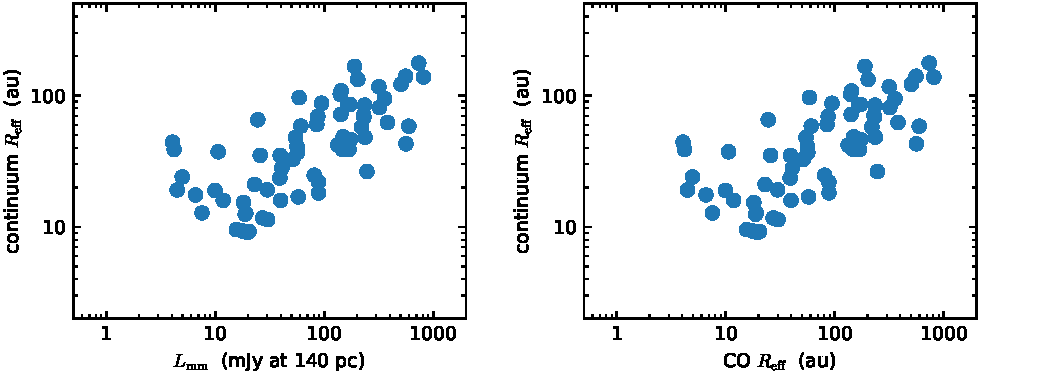
\includegraphics[width=\textwidth]{sizes.pdf}
\caption{(a) The observed correlation between the $\lambda = 0.9$ mm continuum sizes (the effective radii that encircle 68\%\ of the flux density) and luminosities (in flux density units, scaled to a distance of 140 pc), with the inferred $R_{\rm eff} \propto L_{\rm mm}^{0.5}$ scaling relation overlaid (data from \citealt{tripathi17,andrews18}, Hendler et al.~2019).  (b) A comparison of the sizes inferred from the mm continuum and the $^{12}$CO line emission, with markers indicating various levels of discrepancy (data from \citealt{ansdell18} and elsewhere).}
\label{fig:sizes}
\end{figure}


\subsubsection{Caveats and Ambiguities}
The important caveat to such empirical size measurements is that they are not directly (or linearly) tied to the mass distribution.  While their behavior may point to fundamental physical relationships, a translation  into physical radii is not obvious (and indeed does not make much sense).  This is particularly challenging in the comparisons of mm continuum and $^{12}$CO sizes, where optical depth effects and radial opacity variations are important.  Ultimately, a quantitative version of that comparison relies on more detailed radiative transfer calculations; evidence for the size discrepancy is only available in a logical negation of the assumption that $\zeta(r) \approx {\rm constant}$.    



\subsection{Surface Density Profiles} \label{sec:sigma}

In principle, spatially resolved measurements of the same mass tracers introduced in Section \ref{sec:mass} can be used to constrain the radial surface density profiles of the solids ($\Sigma_s$) or gas ($\Sigma_g$).  In simple models for the gas evolution, measurements of $\Sigma_g$ offer insights on the turbulent viscosity (e.g., \citealt{hartmann98,hueso05}) or large-scale winds \citep[e.g.,][]{blandford82,pudritz83,bai13} that regulate the accretion and angular momentum transfer of disk material.  The behavior of $\Sigma_g$ also determines what types of planets and system architectures can be formed \citep[e.g.,][]{miguel11,alibert13}, and how they will evolve via migration \citep[e.g.,][]{paardekooper10,baruteau11}.  Meanwhile, the processes that drive the growth of dust grains into planetesimals are largely dictated by the $\Sigma_s$ profile \citep[e.g.,][]{garaud07,johansen09,birnstiel12}.  It is not an overstatement to claim that the disk density structure ties into all the key physical processes relevant to planet formation.        

\subsubsection{Overview of Measurements}
A key emphasis on the interpretation of modest resolution ($\sim$20--50 au) interferometric observations of the mm continuum morphologies has been on estimating the shape of $\Sigma_s$ \citep{aw07a,pietu07,pietu14,andrews09,andrews10,isella09}.  The mechanics and parameterizations of the modeling used to measure those gradients varies substantially between studies, but a crude distillation of the results in terms of a broken power-law prescription suggests $\Sigma_s \propto r^{-1}$ or shallower in the inner disk, and $\Sigma_s \propto r^{-3}$ or steeper at large radii.  These studies are really measuring the gradients at large distances from the host star (tens to hundreds of au): extrapolations to the inner disk are determined by the functional form of the adopted $\Sigma_s$ parameterization and (at best) a few resolution elements that trace a turnover toward the inner disk.  The inferred $\Sigma_s$ values span $\sim$0.001--1 g cm$^{-2}$ at $r \approx 50$--100 au, comparable to the disk-averaged $\langle \Sigma_s \rangle$ expected from the normalization of the continuum size--luminosity relation and similar assumptions about the temperatures and opacities \citep{tripathi17}.  

Measurements of $\Sigma_g$ from line emission are still relatively rare, due primarily to the weaker emission from optically thin spectral lines.  The basic methodology is similar to the continuum work, where parameterized density prescriptions and thermal structures are forward-modeled to match the resolved interferometric data \citep[e.g.,][]{guilloteau98,isella07,qi08,qi11,rosenfeld13b,williams16}, in some cases with a more sophisticated backend to properly treat realistic abundances from chemical equilibrium models, heating, and molecular excitation \citep[e.g.,][]{woitke09,bruderer14,miotello18}.  Ideally, some of the intrinsic degeneracies can be mitigated by modeling multiple species or transitions of a given tracer molecule \citep[e.g.,][]{dartois03,schwarz16,zhang17,cleeves17}.  Some creative recent methodologies aim to get around the requirement of an assumed tracer abundance, using either excitation constraints from density-sensitive line ratios \citep[e.g.,][]{dutrey17} or multiwavelength continuum size measurements and a simplified model for the aerodynamics of solids embedded in the gas \citep{powell17,powell19}.       


\subsubsection{Caveats and Ambiguities}
The inferences and interpretations of density profiles suffer the same ambiguities outlined for the masses (Section \ref{sec:mass}), although with the added complexity that comes with access to their spatial variations.  Efforts to quantify $\Sigma_s$ are stymied by the evidence that optical depths can be high inside a few tens of au and that $\kappa_\nu$ varies with radius (see Section \ref{sec:solids}).  Analogous concerns limit estimates of $\Sigma_g$ (for the standard approaches).  Moreover, if solid densities are high spectral line emission can be prevented from reaching the observer if it originates below the continuum photosphere or from the back side of the disk \citep[e.g.,][]{weaver18,isella18}.  If that continuum blocking is significant, robust estimates of $\Sigma_g$ from line data will also need to simultaneously infer $\Sigma_s$ from (multiwavelength) continuum data (a daunting prospect).  

\begin{figure}[t]
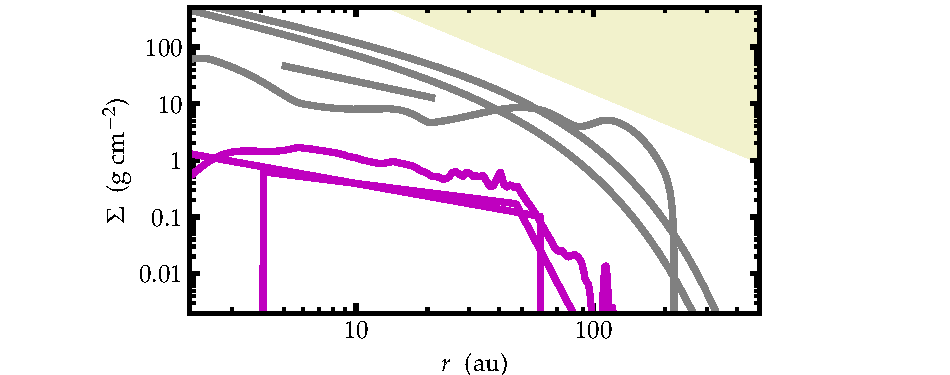
\includegraphics[width=\textwidth]{tw_sigma.pdf}
\caption{tbd}
\label{fig:tw_sigmas}
\end{figure}

It is safe to argue that the ability to quantitatively measure density profiles is still in an exploratory phase, with progress that is severely limited by systematics related both to the methodology and the intrinsic degeneracies.  This is illustrated in {\bf Figure \ref{fig:tw_sigmas}}, which shows the wide range of $\Sigma_g$ and $\Sigma_s$ estimates for the TW Hya disk from various approaches in the literature, along with some standard benchmarks for reference.    

 


\subsection{Opacities and Particle Properties} \label{sec:opacities}

Although not a formal aspect of the disk structure, the microphysical properties of an ensemble of solids -- compositions \citep{pollack94}, sizes \citep{miyake93}, morphologies \citep{henning96} -- are strongly influenced by their local physical conditions, and therefore merit some elaboration.  In a sense, these characteristics are useful, albeit indirect, diagnostics of the disk structure (see Section \ref{sec:solids}).  The particle properties are encoded in the absorption and scattering opacities, and are therefore fundamentally important for interpreting observations of thermal continuum emission.          

%There are large uncertainties in any inference of $M_s$ from microwave continuum data, for two primary reasons.  First, the assertion that the emission is optically thin is unlikely to be valid at all disk locations.  Once optical depths are high, the emission saturates and mass is hidden ($M_s$ is under-estimated).  The significance of this effect depends on the surface area of the thick emission, which will be revisited in various contexts throughout this review.  Second, even in the $\tau_\nu \ll 1$ limit, the continuum luminosity scales with the product of the temperature, opacity, and mass.  The uncertainty in $T$ will be addressed in Section \ref{sec:temp}.  There is considerable ambiguity in $M_s$ estimates due solely to our relative ignorance of the microphysical particle properties that set $\kappa_\nu$, including their mineralogical (and ice) compositions \citep{pollack94}, sizes \citep{miyake93}, and internal structure (porosity; \citealt{henning96}).  

Information about the compositions of disk solids can be accessed through spectral features in the infrared, particularly from silicates \citep{kessler-silacci06,bouwman08,sargent09b} and common ices \citep{oberg08,bottinelli10,mcclure15}.  Various carbonaceous materials are also expected to be primary constituents \citep{zubko96,jaeger98}.  The implied compositions are commensurate with {\it in situ} measurements of dust particles, meteorites, and larger ``primordial" bodies in the Solar System \citep[e.g.,][]{clayton04,mumma11}.  The sizes and morphologies of the emitting particles have the most pronounced effects on the behavior of the opacities.  Size distributions are often approximated as power-laws, $n(a) \propto a^{-q}$ for size (radius) $a \in [a_{\rm min}, a_{\rm max}]$, with indices comparable to the expectation for a self-similar collisional cascade ($q \approx 3.5$; \citealt{dohnanyi69,tanaka96}) or more top-heavy variants ($q \approx 2.5$; e.g., \citealt{birnstiel11}).  The particle morphologies are characterized by their porosities, usually parameterized with a volume filling factor $f_s$ ($\sim$1 for compact particles, but can be as low as $\sim$10$^{-4}$ in aggregates; \citealt{kataoka13}).  The mm opacity spectrum is roughly a power-law, $\kappa_\nu \approx \kappa_0 (\nu/\nu_0)^\beta$, where $\kappa_0$ and $\beta$ both depend on \{$q$, $a_{\rm max}$, $f_s$\}.  

For reference, {\bf Figure \ref{fig:opac}} illustrates how the opacities respond to particle properties, for some representative model variations (see \citealt{cuzzi14}, \citealt{woitke16}, or \citealt{dsharp5} for more detailed explorations of the parameter-space). When $a_{\rm max} \ll \lambda$, the absorption opacity normalization, $\kappa_0^{\rm abs}$, is roughly independent of the size cut-off, $\beta$ is high ($\sim$1.7, as for the small dust grains in the interstellar medium; \citealt{finkbeiner99}), and scattering is negligible (the albedo $\omega_\nu \approx 0$).  When $a_{\rm max} \gg \lambda$, $\kappa_0^{\rm abs}$ decreases with $a_{\rm max}$ at a rate that depends on $q$ (lower $q$ means a steeper fall-off; e.g., \citealt{ricci10a}), $\beta$ is lower (scaling roughly with $q$; \citealt{draine06}), and albedos depend on $q$ (large $q$ implies higher $\omega_\nu$).  When $a_{\rm max} \sim \lambda$, resonances drive up $\kappa_0^{\rm abs}$, $\beta$, and $\omega_\nu$.  Porosity dampens those resonant amplifications in the absorption opacities, but can enhance albedos \citep{kataoka14}.  
% consider swapping notation to have albedo = eta (not omega); that's what Birnstiel does (check what Draine
% and other folks do)
%Specifically, $\kappa_0^{\rm abs}$ varies with the product $a_{\rm max} f_s$, such that porous particles have a lower $\kappa_0^{\rm abs}$ and higher $\beta$ than compact particles with the same size distribution \citep{kataoka14}.  %%% SA: this is clearly not generically true (or true in detail)!

\begin{figure}[t]
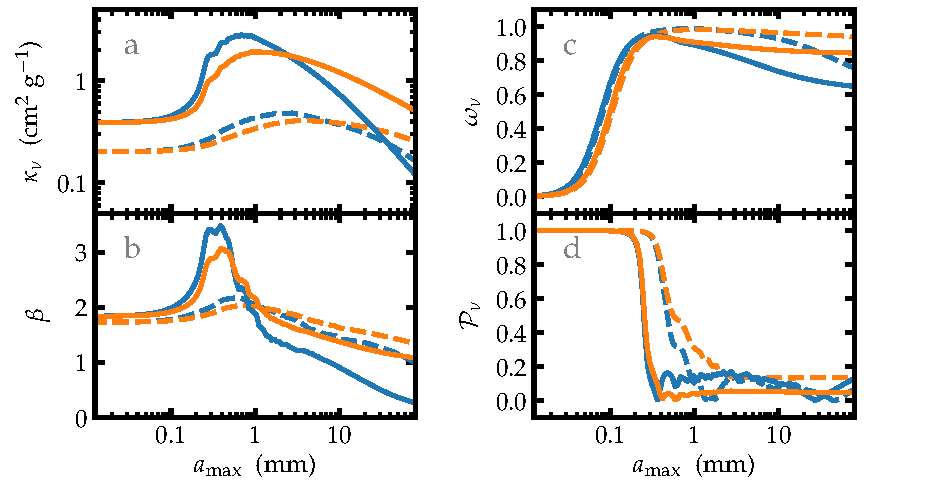
\includegraphics[width=\textwidth]{opac.pdf}
\caption{kappa0, beta, albedo as fn of amax (different q, phi, composition, mixing rule, DDA v Mie)}
\label{fig:opac}
\end{figure}

\subsubsection{Overview of Measurements}
Access to information about the opacities comes from thermal continuum emission from the particles, as described in Section \ref{sec:primer_cont}.  Even if optically thin, the continuum emission intensity cannot directly constrain $\kappa_0^{\rm abs}$ because of the degeneracy with $\Sigma_s$.  Instead, information about the particle properties are primarily accessible from the shape (or ``color") of the mm continuum spectrum, $\alpha_{\rm mm}$, presuming all of the emission is optically thin.  Multiwavelength photometry surveys find disk-averaged $\langle \alpha_{\rm mm} \rangle \approx 2$--3 \citep{beckwith91,mannings94,ricci10a,ricci10b,ricci12}, implying $\langle \beta \rangle \le 1$ and $\langle a_{\rm max} \rangle \gtrsim 1$ mm.  {\bf Figure \ref{fig:opac}} also shows how $\langle \alpha_{\rm mm} \rangle$ varies with $L_{\rm mm}$ and $R_{\rm mm}$.  Spatially resolved inferences of $\alpha_{\rm mm}$ typically show a radial increase from $\sim$2 to $\gtrsim$3, typically interpreted as evidence that particle sizes are considerably larger at smaller disk radii ($a_{\rm max}$ decreases from a few cm to sub-mm sizes; e.g., \citealt{perez12,lperez15,menu14,tazzari16}; see Section \ref{sec:solids}). 

Complementary insights on particle sizes are available from the polarization of self-scattered sub-mm/mm continuum emission \citep{hughes09b,kataoka15}.  Albedos increase sharply at $a_{\rm max} \sim \lambda / 2\pi$ (see {\bf Figure \ref{fig:opac}}), while the polarization fraction exhibits the opposite behavior.  The net effect implies that the wavelength dependence of the polarization fraction sets a stringent limit on $a_{\rm max}$.  Resolved observations of the sub-mm/mm polarization morphology are consistent with model predictions for scattering \citep{kataoka16a,yang17,stephens17,hull18,bacciotti18,dent19}.  The few disks with measured multiwavelength polarization fractions indicate that $a_{\rm max}$ is in the sub-mm range \citep[e.g.,][]{kataoka16b,ohashi18}.  

%,  presuming scattering is the dominant polarization mechanism.        

\subsubsection{Caveats and Ambiguities}
There are both technical and observational ambiguities associated with the particle properties.  On the technical side, the conversion of the physical characteristics of the particles into their corresponding optical properties is important, and could be considerably more complicated than is often assumed.  Some of these key issues include accounting for the temperature dependence of the constituent refractive indices, the methodology adopted for mixing those dielectric properties in a composite particle, appropriately calculating absorption and scattering cross sections of porous, non-spherical particles, and the over-simplified assumption of a single power-law size distribution, to name only a few (for more details, see the discussion by \citealt{dsharp5}).   

Putting aside these technical issues, there are some general systematic uncertainties associated with interpreting observational diagnostics of the particle properties.  There is a sort of apocryphal notion that optically thin continuum emission traces particles with a size comparable to the observing wavelength: a more accurate statement is that the emission is most efficient with this criterion, since it corresponds to the peak $\kappa_0^{\rm abs}$ (giving the most emission per mass).  However, particles of all sizes still contribute, and that facilitates the fundamental ambiguity that the opacities can be arbitrarily low if large solids are present.  The key practical point is that a constraint on $\beta$ from a measurement of $\alpha_{\rm mm}$ only sets a lower bound on $a_{\rm max}$, since $\beta$ saturates once $a_{\rm max} \gg \lambda$ (see {\bf Figure \ref{fig:opac}}).  That, in turn, sets an upper bound on $\kappa_0^{\rm abs}$, and correspondingly a lower bound on $\Sigma_s$ (or $M_s$).  
\begin{marginnote}
Note in {\bf Figure \ref{fig:opac}} that the opacities routinely adopted in the literature ($\sim$2 cm$^2$ g$^{-1}$ at $\lambda = 1.3$ mm) are effectively upper bounds. 
\end{marginnote}

The presence of optically thick emission severely complicates the interpretations of these diagnostics of the particle properties (see Section \ref{sec:primer_cont}).  Low $\alpha_{\rm mm}$ values could alternatively be attributed to high optical depths, even if nominally the filling factor is rather modest \citep[e.g.,][]{ricci12}.  The preferentially flatter spectra inferred at smaller disk radii from resolved multiwavelength data could instead be attributed to optically thick inner disks, with $\alpha_{\rm mm}$ there being more of a diagnostic of the spectral variation of the albedo \citep{zhu19,liu19}.  That scenario may help reconcile the mild tension between the particle sizes inferred from $\alpha_{\rm mm}$ and the polarization fractions, and could then offer a tight constraint on the particle sizes in the continuum photosphere layer.  Well-resolved, multiwavelength polarization measurements would be crucial in this regard, since there are plausible alternative mechanisms for polarizing the continuum \citep[e.g.,][]{matsakos16,stephens17,tazaki17,yang19,kataoka19}; though with peak polarization fractions of a few percent, this is a challenging observational task.            
%key problem is that low spectral index can also mean optically thick, although nominally with modest filling factor.  it sort of depends on how optically thick emission is distributed though (ricci).  spatially resolved alpha might point out that inner disk is thick.

%polarization signatures can be induced by other mechanisms; ideally want higher resolution view at many wavelengths to understand better (but that's hard with ~few percent pol levels).  one possible solution to apparent tension in amax estimates is to have an optically thick photosphere with just the right particle sizes to get v high albedos, right pol, and then sub-planckian emission to give you wonky alphamm.

%Unresolved spectral index measurements naturally gloss over some important complexities.  The particle properties, and thereby the opacities, are expected to vary spatially in disks.  The (presumably inter-dependent) morphologies of those variations make it difficult to determine the impact of $\kappa_\nu$ changes on inferences of $M_s$ without spatially resolved measurements of $\alpha_{\rm mm}$.  Moreover, an unknown fraction of the continuum emission can be optically thick, where $\alpha_{\rm mm} \approx 1.5$--2.5 depending on $T$ (or $\alpha_{\rm Pl}$) and the spectral dependence of the albedo \citep{zhu19,liu19}.  This would diminish unresolved (disk-averaged) estimates of $\beta$, again limiting an assessment of the $M_s$ uncertainty due to the opacities.



%honest assessment: the only robust way to do this is long term: model resolved multi-line emission, rely on iterative self-cal of chemical models, etc.  painful, but could illuminate a path forward with (a) some effort here and (b) some more datasets that may point to important patterns.


\subsection{Thermal Structure} \label{sec:temp}

The thermal structure of a disk helps determine the distribution and evolution of its constituent material.  Its role is usually distilled in terms of a fundamental kinematic scale, the sound speed $c_s$ ($\propto \sqrt{T}$), or a related spatial scale, the gas pressure scale height $H_p = c_s / \Omega_{\rm k}$ ($\propto \sqrt{T r^3}$) where $\Omega_{\rm k}$ is the Keplerian angular velocity.  Irradiation by the host star is the primary factor determining the temperature distribution.  Small dust grains in the disk atmosphere absorb starlight efficiently (due to their large $\kappa_\nu^{\rm abs}$ in the infrared), and re-radiate some of that energy deeper into the disk \citep[e.g.,][]{chiang97,dalessio98}.  The net results are an increasing $T(z)$ \citep{calvet91} and a decreasing $T(r)$ \citep{kenyon87,adams90}.  This heating mechanism depends on the host star spectrum and luminosity ($L_\ast$), as well as the microphysical properties (see Section \ref{sec:opacities}) and vertical distribution of the particles, which dominate the opacity \citep{dalessio99b,dalessio06,dullemond02,dullemond04b}.  The height at which starlight is absorbed is set by the balance between turbulent diffusion (vertical mixing), particle growth, and the coupling of solids to the hydrostatic support of the gas \citep{dubrulle95,turner10}.  If all else is equal, more vigorous mixing or a smaller $z$-component of the gravity (relative to the pressure) increases the height (and therefore irradiated area) of this surface layer, which in turn leads to a warmer disk.  

Since the molecular excitation and thermal emission in both spectral lines and the mm continuum depend so intimately on the temperature distribution, it is important to consider additional contributing factors to the disk heating and cooling.  For example, some spectral line emission originates in locations where $\zeta$ is low (e.g., high in the disk atmosphere or at large radii; see Section \ref{sec:solids}) and the broadband continuum cooling is therefore diminished; then, collision rates can be low enough that the gas is super-heated ($T_g > T_s$; e.g., \citealt{jonkheid04,kamp04,bruderer13}).  And, while usually secondary to stellar irradiation, alternative heating sources -- viscous dissipation \citep{shakura73,dalessio98}, spiral shocks \citep{rafikov16}, radioactivity \citep[e.g.,][]{cleeves13}, external irradiation (e.g., from an envelope; \citealt{dalessio97}) -- or other perturbations (e.g., self-shadowing; \citealt{dullemond04a}) to the thermal structure of a disk can still play important physical and observational roles.  


\subsubsection{Overview of Measurements}
Optically thick tracers offer superior constraints on the thermal structure in disks.  The classical approach is to forward-model the spatially unresolved infrared spectral energy distribution (SED) with a reasonable density (and opacity) prescription, because its shape and amplitude are sensitive to the gradient and normalization of $T(r)$ in the photosphere layer, respectively \citep{adams90,chiang97,dalessio98}.  Some additional constraints are available from scattered light or mm continuum images that resolved the vertical structure of the disk, particularly for edge-on viewing geometries \citep[e.g.,][]{stapelfeldt98,lee17}.

The radial intensity profile of an optically thick spectral line is sensitive to the temperature distribution at the height of the (vertically narrow) line photosphere \citep[e.g.,][]{beckwith93,dutrey14,weaver18}.  With sufficient resolution, the two dimensional geometry of that specific emission layer can be measured direcly (e.g., \citealt{rosenfeld13a,pinte18}, Dullemond et al.~2019).  In principle, an empirical constraint on $T(r,z)$ is possible by probing the temperature profiles at different depths in the disk atmosphere with multiple transitions (or other tracer lines) with a range of excitation conditions \citep[e.g.,][]{dartois03,qi04,schwarz16}.  Ideally, that multi-line reconstruction effort can be supplemented with discrete benchmarks in $T(r)$ that are accessible from chemical signposts of condensation fronts (snowlines), where major volatile species (CO, N$_2$) are removed from the gas phase when they freeze onto particle surfaces (e.g., \citealt{qi11,qi13,qi15}, Qi et al.~2019).    


\subsubsection{Caveats and Ambiguities}
The fundamental challenge in measuring disk temperatures, particularly from continuum emission, are the intricate physical degeneracies involved.  For example, the optical properties (and thereby opacities) of the particles are $T$-dependent \citep[e.g.,][]{boudet05,demyk17}, but the temperatures are set by the local variations in $\kappa_\nu$.  Treating this complexity in a self-consistent way is a computational challenge, and even when successful requires a curtailed model sophistication for tractability \citep[e.g.,][]{woitke16}.  The resulting ambiguity somewhat limits the power of temperature constraints from continuum measurements \citep[e.g.,][]{heese17}.  

There are few successful examples of the spectral line approach for $T(r,z)$ measurements in disks, primarily because collecting data for the different tracers demands a substantial observational investment.  The primary challenge is achieving appropriate sensitivity at high resolution, although there are more technical concerns related to continuum contamination \citep{weaver18} and non-LTE excitation.  However, a compromise in data quality might be compensated with a sufficient volume of different tracers \citep[e.g.,][]{fedele16}.  Ultimately, this approach is essentially a requirement for robust constraints on the disk structure: only once a data-based $T(r,z)$ model is available can optically thin spectral line measurements facilitate estimates of the gas densities.



\subsection{Dynamics and Structure} \label{sec:turb}
All of the key structure properties outlined above are heavily influenced by the dynamics of the gas disk.  The dynamical structure of this fluid controls the transport of mass and angular momentum in the disk, and thereby determines the evolution of its density distribution.  The dynamical coupling between the gas and solids is fundamental to planet formation, since it plays crucial roles in particle growth from dust grains to planetesimals and beyond (Section \ref{sec:solids}).  The dominant contribution to the dynamics of a parcel of gas is its orbital motion around the host star.  But deviations from that Keplerian velocity field ($v_{\rm k}$) are expected, due to effects like pressure support, self-gravity, winds and outflows, magnetohydrodynamic (MHD) flows, and viscous transport.  

Beyond these factors that control the ordered dynamical structure of a disk, there is special interest in  random motions.  Turbulence has traditionally been asserted as the origin of the disk viscosity that facilitates angular momentum transport (and ultimately accretion onto the host star), drives chemical mixing, and sets the relative velocities of solids, among other diffusive processes.  The amount of turbulence is usually characterized in terms of a dimensionless coefficient, $\alpha_{\rm t} = \nu / c_s H_p$, where $\nu$ is the fluid viscosity.  For traditional models of turbulence driven by the magnetorotational instability (MRI), the expectation is $\alpha_{\rm t} \sim 0.001$--0.01.  But a shifting theoretical paradigm now argues that the MRI is suppressed over much of the disk volume by non-ideal MHD effects, suggesting that turbulence (and viscous transport itself) is minimal, with an effective $\alpha_{\rm t} \lesssim 10^{-4}$.  


\subsubsection{Overview of Measurements}
A tomographic reconstruction of the disk velocity field is possible with a collection of spatially and spectrally resolved maps of emission lines with a variety of optical depths.  The process is conceptually similar to deriving the thermal structure (Section \ref{sec:temp}), but with a focus on the kinematic pattern rather than the line intensities.  That said, the same limitations on sensitivity and resolution have made suitable datasets rare.  The available data confirm only that orbital motions are dominant \citep{simon00,msimon17,rosenfeld12,czekala15,czekala16}.  Deviations from Keplerian motions are expected at the few percent level at radii of tens to hundreds of au \citep{rosenfeld13a}.  Recently, some kinematic signatures of winds \citep[e.g.,][]{guedel18} and small-scale pressure modulations \citep{yen16,teague18a,teague18b,pinte18b} have been teased out from emission line maps of especially bright targets.  

Constraints on turbulence are available from a few different observational probes.  First, and most direct, is a resolved measurement of spectral line broadening since the linewidth is set by the composite distribution of thermal (with characteristic width $(k T / m)^{0.5}$ for molecular mass $m$) and non-thermal (with width $\delta v_{\rm t}$) motions.  Constraints on $\delta v_{\rm t}$ are available for only three examples.  In two cases only upper limits are identified from various CO, CS, and DCO$^+$ lines that probe radial scales of $\gtrsim$50--100 au and heights of $\sim$1--3 $H_p$, with $\delta v_{\rm t} < 0.03$--0.08 $c_s$ or $\alpha_{\rm t} \lesssim 0.002$--0.007 \citep{hughes11,flaherty15,flaherty17,flaherty18,teague18a}.  The third case finds a much broader CS linewidth, $\delta v_{\rm t} \approx 0.6$ $c_s$ ($\alpha_{\rm t} \approx 0.4$), at similar radial and vertical scales, although the adopted prescription for converting the broadening measurement into a turbulence constraint may be inappropriate in that case \citep{guilloteau12}.   

% TW Hya from Flaherty+ 18: dv < 0.1 cs at 2-3 Hp (alpha < 0.007) from CO 2-1.
%             Teague+ 18 agrees based on CS lines
%             Hughes+ 11 numbers are only slightly less stringent (if at all) from CO 3-2
% HD 163296 from Flaherty+ 17: dv < 0.05 cs (alpha < 0.003) from CO 2-1, C18O 2-1, DCO+ 3-2 
%                Flaherty+ 15: dv < 0.03 cs (alpha < 0.002) from CO 3-2 and other CO 2-1 isotopologues
%                Hughes+ 11 found a marginal detection that must be wrong
% DM Tau from Guilloteau+ 12: dv ~ 0.6 cs (alpha ~ 0.4 !?) from CS 3-2 at ~2-3 Hp

second, can quantify diffusion based on nominally ``sharp" features.  for example, the radial widths (dullemond) or vertical heights (pinte) of dust continuum features are connected to turbulent mixing processes.  discuss constraints / upper limits in context of alpha.  mention Owen's snowline idea.  point out that both types of measurement suggest that turbulence is low, alpha < 1e-3ish, consistent with concept that MRI is suppressed over most of the disk volume due to non-ideal MHD effects.


\subsubsection{Caveats and Ambiguities}
Inferring that turbulent contribution from interferometric observations of a molecular emission line are a challenge, primarily because the thermal term dominates.
same issues with line measurements, and limited resolution can cause you to screw up your v-field reconstruction if you do not know the line photosphere location.  there's some special ambiguities due to warps.  structural perturbations are secondary effects; they matter at the per cent level.  that also implies they are not easy to separate from the dominant rotation field (though teague, yen have worked on ways to do this properly).

line broadening measurements are difficult, because there is a direct degeneracy with the (poorly constrained) thermal structure of the line-emitting region.  that introduces some ambiguity, but the fact remains that no evidence for turbulent broadening is found (limits might change a bit).  the degeneracies of the continuum-based diffusion constraints are orthogonal: they depend on the sizes of the particles responsible for the continuum emission.  fact that they agree in scale with the line broadening limits suggests that the conclusion of little turbulence is robust, even if precision is still lacking.  
 

%\begin{figure}[h]
%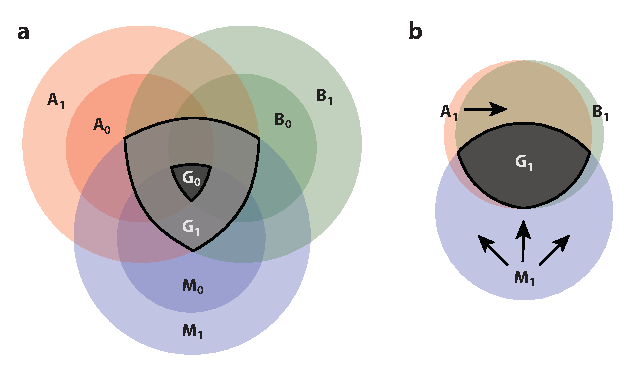
\includegraphics[width=3in]{SampleFigure}
%\caption{Figure caption with descriptions of parts a and b}
%\label{fig:continuumstuff}
%\end{figure}


\begin{textbox}[h]\section{Summary}
TBD  
\end{textbox}


%\subsection{Dynamics}
%turbulence; the dynamical impact of non-ideal MHD terms; accretion flows

%\subsection{Summary}




\section{DEMOGRAPHIC\ INSIGHTS} \label{sec:demographics}
some flowery introduction.


\subsection{Links to Host Properties}
somehow triggered to think that disk masses are tied to host masses.  naive gravitational intuition.  in reality, there is no need for this to be true, at least at the typical ages for which we measure disk masses, since it all depends on early evolution (accretion, etc.).  nonetheless, there are indirect hints based on connections made in the exoplanet population (run through that conceptually).

as continuum surveys expand their dynamic range in both mhost and lmm, found hints for a correlation.  quantitatively characterize this.  comment on deviations between surveys.  some of the differences are more tied to how one interprets the lmm -to- ms connection (describe why), but similar behavior in lmm - mhost only.  comment on scatter origins -- multiplicity, evolution, temperature, opacity, density structures, and sizes are possibilities.  not yet clear if line emission diagnostics of Mg scale too, although some hints that line and continuum luminosities scale.

growing information on connection between mhost and disk sizes.  any correlation is quite weak, although that is to be expected based on the mhost - lmm and lmm - size relations (quantify these things).  

its compelling to note that the scalings seem a bit tighter with lstar compared to mstar.  hard to know what the real dependent variable is, since most of the sample is roughly co-eval with a single stellar mass-lum relation.  describe how in any case the only way you can get these relationships is if there is an intrinsic scaling between the host mass/lum and the disk size (or continuum size).  

too limited to address connection to gas disk sizes, although rafikov and najita like to make the leap because of potential connections to viscous evolution.  some of that is motivated by connections to accretion rates.  discuss manara and mulders results.  again, not clear if the fundamental relation is the mhost - mdot relation or the mhost - mdisk relation...but because of the inter-connections, the other always follows.


\subsection{Environmental Effects}

two key environmental effects, on local scales/``internal" (multiplicity) and global scales/``external" (stripping via tidal encounters or harsh irradiation from nearby massive stars).  


\subsubsection{Multiplicity}
basic mechanics of disk truncation idea.  field population multiplicity rates and separation/eccentricity distributions.  differences there for nearby low-mass clusters.  that implies an expectation that multiplicity is pretty important in shaping observables.  see evidence for diminished continuum luminosities for pairs with closer separations (projected).  weird CB disk exception.  

primaries have more mass in majority, but not all, cases.  population of stars in multiples follows similar scaling with host mass.  there is not good evidence for a continuum size vs separation relationship predicted by theory; maybe partly due to not using gas as the tracer, but could also be related to evidence for non-coplanarity (discuss that).  worth noting that fainter disks at smaller separations does not necessarily imply lower densities (consider how much emission you would get for v small optically thick disks).  FIGURE: show separation-Lmm distribution for all available pairs (maybe in left panel of 2-panel figure).


\subsubsection{Close Encounters}
natural extension of tidal truncation in multiple systems is the effect of close, one-time encounters in a dense cluster environment.  this is generally though to be rare in the diffuse T associations where work has focused so far, but might actually be comparatively frequent because most stars are born in much denser/richer clusters.  general evidence is now limited by this selection bias, although there are a few compelling test examples nearby that conform with general tidal truncation expectations.  


\subsubsection{External Photoevaporation}
need to catch up.  FIGURE: probably second panel here showing Lmm versus distance from theta1 Oric.



\subsection{Evolutionary Signatures}


\subsection{Summary}


\section{THE\ EVOLUTION\ OF\ DISK\ SOLIDS} \label{sec:solids}

%The standard assumption is that solids contribute a small fraction, $\sim$1\%, of the total mass budget in a disk.  Even in that case, solids play outsized roles in disks by helping to regulate their thermal balance (as the dominant opacity source) and facilitating complex chemical networks (as the sites of ice-modulated reactions), among other things.  Perhaps most significantly, disk solids are ultimately the seeds for the formation of planets.  As points of reference, the current census of exoplanets indicates that ``rocky" worlds are especially common \citep[e.g.,][]{howard10,dressing13,malhotra15}, and {\it in situ} measurements indicate that the giant planets in our Solar System contain massive sold cores \citep{saumon04,bolton17}.  Constraints on the spatial distribution of solids are essential for developing models of disk physics, and would be crucial resources for understanding the first steps of the planet formation process. 

\subsection{Particle Growth and Migration}
 

\subsection{Observational Constraints and Conundrums}

% polarization: albedo limits sizes of mm scatterers to ~100um


\subsection{Summary}



\section{SUBSTRUCTURES} \label{sec:substructures}

\subsection{Impact of Pressure Modulations}

\subsection{Potential Origins}

\subsection{``Transition" Disks}

\subsection{``Normal" Disks}

\subsection{Summary}


\section{SYNOPSIS} \label{sec:summary}

%commentary on ``missing mass" arguments (najita/kenyon, greaves, manara).


\section{FUTURE\ PROSPECTS} \label{sec:future}


\begin{figure}[h]
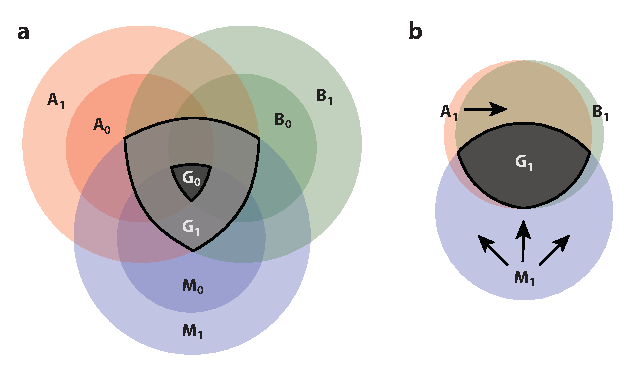
\includegraphics[width=3in]{SampleFigure}
\caption{Figure caption with descriptions of parts a and b}
\label{fig1}
\end{figure}

% Example of a Table
%\subsection{Tables} Tables should also be cited in the main text in chronological order (\textbf {Table \ref{tab1}}).

%\begin{table}[h]
%\tabcolsep7.5pt
%\caption{Table caption}
%\label{tab1}
%\begin{center}
%\begin{tabular}{@{}l|c|c|c|c@{}}
%\hline
%Head 1 &&&&Head 5\\
%{(}units)$^{\rm a}$ &Head 2 &Head 3 &Head 4 &{(}units)\\
%\hline
%Column 1 &Column 2 &Column3$^{\rm b}$ &Column4 &Column\\
%Column 1 &Column 2 &Column3 &Column4 &Column\\
%Column 1 &Column 2 &Column3 &Column4 &Column\\
%Column 1 &Column 2 &Column3 &Column4 &Column\\
%\hline
%\end{tabular}
%\end{center}
%\begin{tabnote}
%$^{\rm a}$Table footnote; $^{\rm b}$second table footnote.
%\end{tabnote}
%\end{table}

% Example of lists
%\subsection{Lists and Extracts} Here is an example of a numbered list:
%\begin{enumerate}
%\item List entry number 1,
%\item List entry number 2,
%\item List entry number 3,\item List entry number 4, and
%\item List entry number 5.
%\end{enumerate}

%Here is an example of a extract.
%\begin{extract}
%This is an example text of quote or extract.
%This is an example text of quote or extract.
%\end{extract}

%\subsection{Sidebars and Margin Notes}
% Margin Note
%\begin{marginnote}[]
%\entry{Term A}{definition}
%\entry{Term B}{definition}
%\entry{Term C}{defintion}
%\end{marginnote}

%\begin{textbox}[h]\section{SIDEBARS}
%Sidebar text goes here.
%\subsection{Sidebar Second-Level Heading}
%More text goes here.\subsubsection{Sidebar third-level heading}
%Text goes here.\end{textbox}



%\subsection{Equations}
% Example of a single-line equation
%\begin{equation}
%a = b \ {\rm ((Single\ Equation\ Numbered))}
%\end{equation}
%Example of multiple-line equation
%Equations can also be multiple lines as shown in Equations 2 and 3.
%\begin{eqnarray}
%c = 0 \ {\rm ((Multiple\  Lines, \ Numbered))}\\
%ac = 0 \ {\rm ((Multiple \ Lines, \ Numbered))}
%\end{eqnarray}

% Summary Points
\begin{summary}[SUMMARY POINTS]
\begin{enumerate}
\item Summary point 1. These should be full sentences.
\item Summary point 2. These should be full sentences.
\item Summary point 3. These should be full sentences.
\item Summary point 4. These should be full sentences.
\end{enumerate}
\end{summary}

% Future Issues
\begin{issues}[FUTURE ISSUES]
\begin{enumerate}
\item Future issue 1. These should be full sentences.
\item Future issue 2. These should be full sentences.
\item Future issue 3. These should be full sentences.
\item Future issue 4. These should be full sentences.
\end{enumerate}
\end{issues}

%Disclosure
\section*{DISCLOSURE STATEMENT}
The author is not aware of any affiliations, memberships, funding, or financial holdings that
might be perceived as affecting the objectivity of this review. 

% Acknowledgements
\section*{ACKNOWLEDGMENTS}
Acknowledgements, general annotations, funding.
% ACKNOWLEDGMENTS: Seba Perez (for HD 169142 images), Roy van Boekel (for TW Hya image), Jane Huang (for TW Hya images), Til Birnstiel (for help with DSHARP opacity software), James Owen (for advice on reviews), David Wilner (sounding board), Kevin Flaherty (thoughts on turbulence),  




\bibliography{references}

\end{document}
